\begin{figure}[!h]
	\centering
	\subbottom[original aerial image\label{fig:arbfrseg}]{
		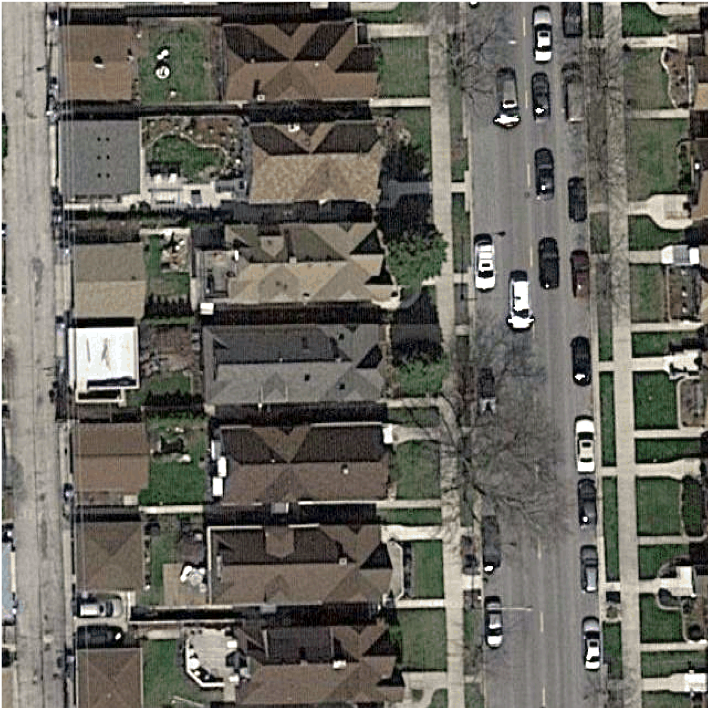
\includegraphics[width=\figfigfig\textwidth]{1-01-0.png}
	}
	\subbottom[semantic segmentation\label{fig:arsemseg}]{
		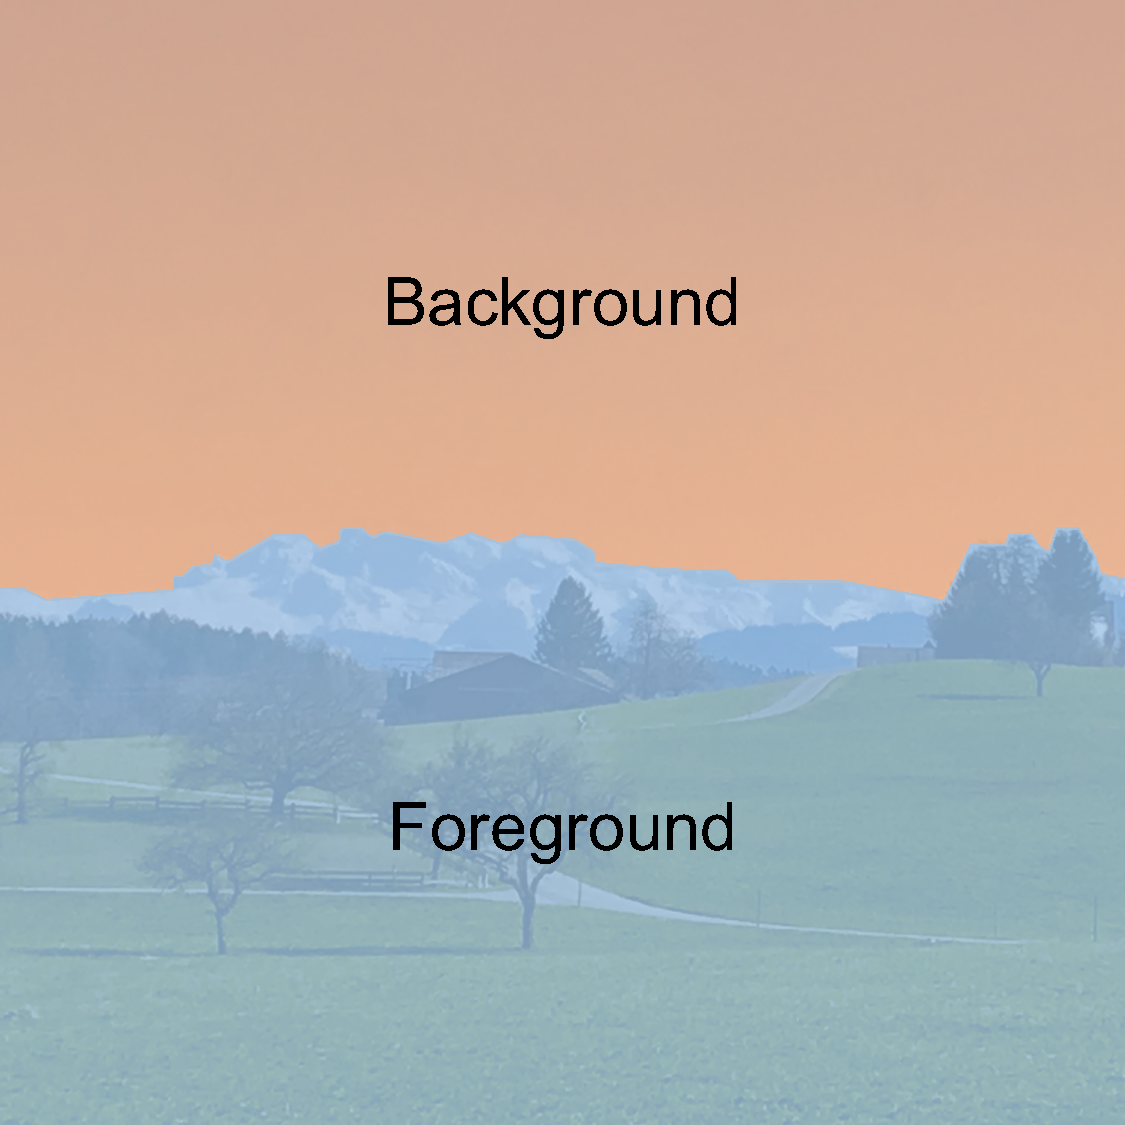
\includegraphics[width=\figfigfig\textwidth]{1-01-1.pdf}
	}
	\subbottom[instance segmentation\label{fig:arinsseg}]{
		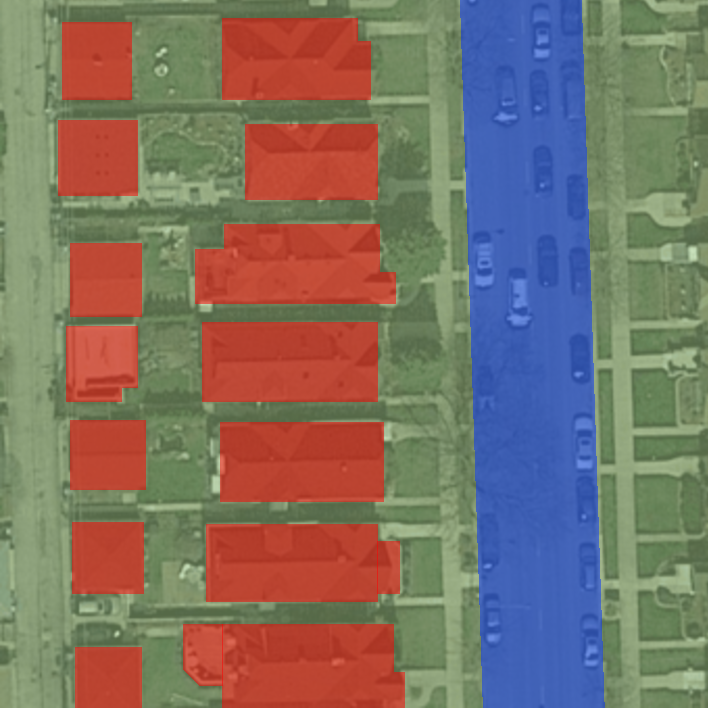
\includegraphics[width=\figfigfig\textwidth]{1-01-2.pdf}
	}
    \caption[Examples of semantic and instance segmentation in aerial image]{Examples of semantic segmentation and instance segmentation in aerial image. The original aerial image (a) is a tile of city Chicago. (b) is the semantic segmentation result of (a), where red color denotes the buildings, blue color denotes the roads, green color denotes the background. (c) is instance segmentation result of (a), where all buildings have the same label, but different ``ID" numbers which can be used to indicate they are different instances.}
	\label{fig:arseg}
\end{figure}